% Niveau :      PCSI *
% Discipline :  Chimie Orga
% Mots clés :   Stéréochimie

\begin{exercise}{Couplage \textit{J} dans les diènes}{3}{PCSI}
{Chimie organique I,Spectroscopie,RMN,Stéréochimie}{bermu}

\begin{questions}
\questioncours Couplage spin-spin $^{2}J$, $^{3}J$ et $^{4}J$ en RMN du proton $^{1}$H. \\
On prendra soin d'expliquer l'origine du phénomène sur un exemple simple et d'énoncer des facteurs d'influence de la valeur de $J$.

\begin{EnvUplevel}
On s'intéresse par la suite au couplage spin-spin dans les diènes conjugués à 6 carbones $\mathrm{C_6H_{10}}$

\begin{center}
    \chemfig{X-[1](-[3]X)=[-1](-[-3]X)-[1](-[3]X)=[-1](-[-3]X)-[1]X},
\end{center}
où X désigne un hydrogène ou groupe méthyle.

Les spectres RMN de ces espèces sont donnés dans l'annexe ci après.
\end{EnvUplevel}

\question Lister les isomères \underline{de constitution} de la forme donnée et donner leur nomenclature IUPAC.

\question Pour chaque isomère, établir quels spectres RMN peuvent (ou non) lui correspondre.

\question Parmi ces isomères, combien donnent lieu à des stéréoisomères \underline{de configuration} ? \\
Lister les différents stéréodescripteurs possibles pour chaque isomère de constitution.

\uplevel{Pour attribuer à chaque stéréoisomère un spectre, nous allons nous intéresser aux couplages $J$.}

\question Retrouver dans la mesure du possible les couplages $J$ du signal ddd dans le spectre \textbf{(\textit{a})}. \\
Pourquoi on ne peut pas retrouver tous les couplages ?

\question Essayez dans la mesure du possible d'attribuer pour chaque stéréodescripteur le spectre qui lui est associé. On pourra s'aider de l'annexe du handbook.
\end{questions}

\end{exercise}

\cleardoublepage

\subsection*{Annexe : spectres RMN $^{1}$H des diènes}

\begin{center}
    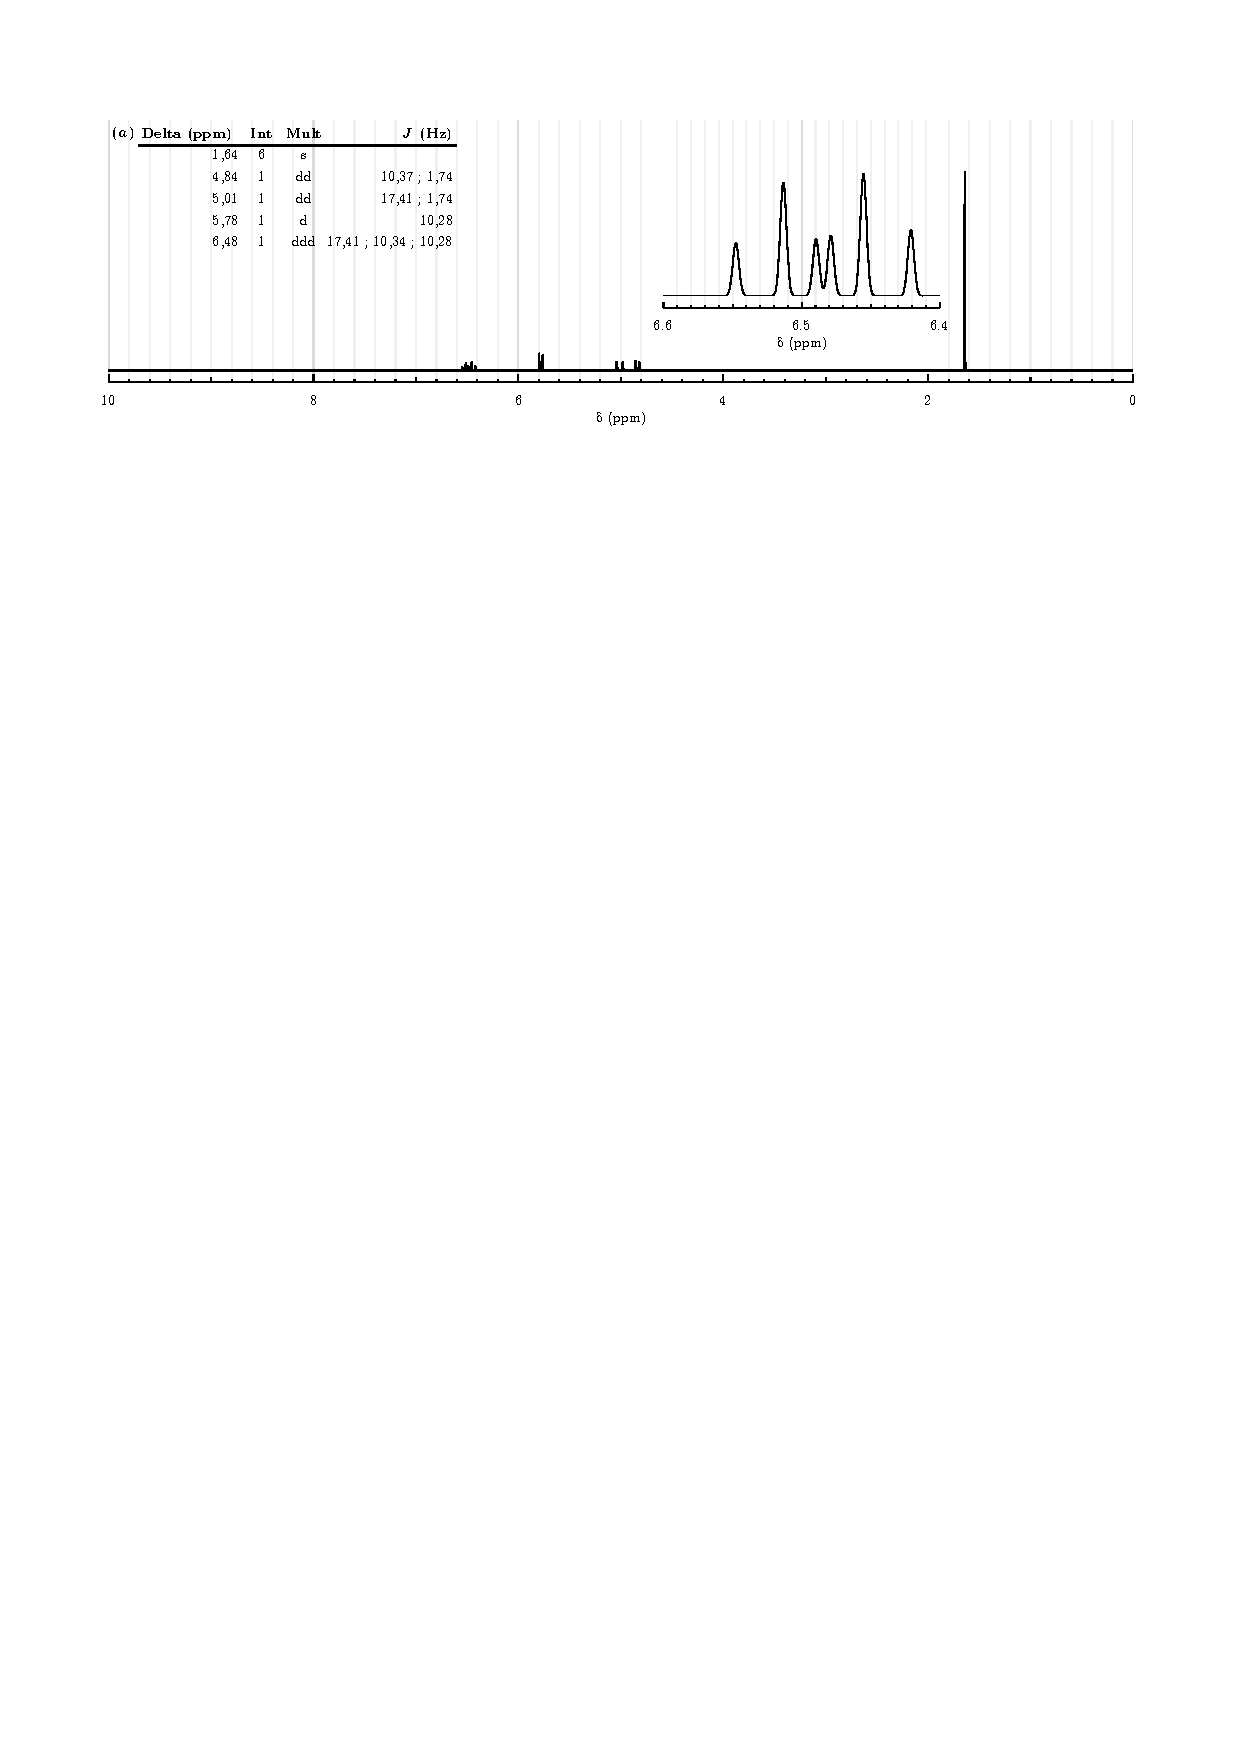
\includegraphics[width=.95\linewidth]{chimiePC/orga/RMN_4met.pdf}
    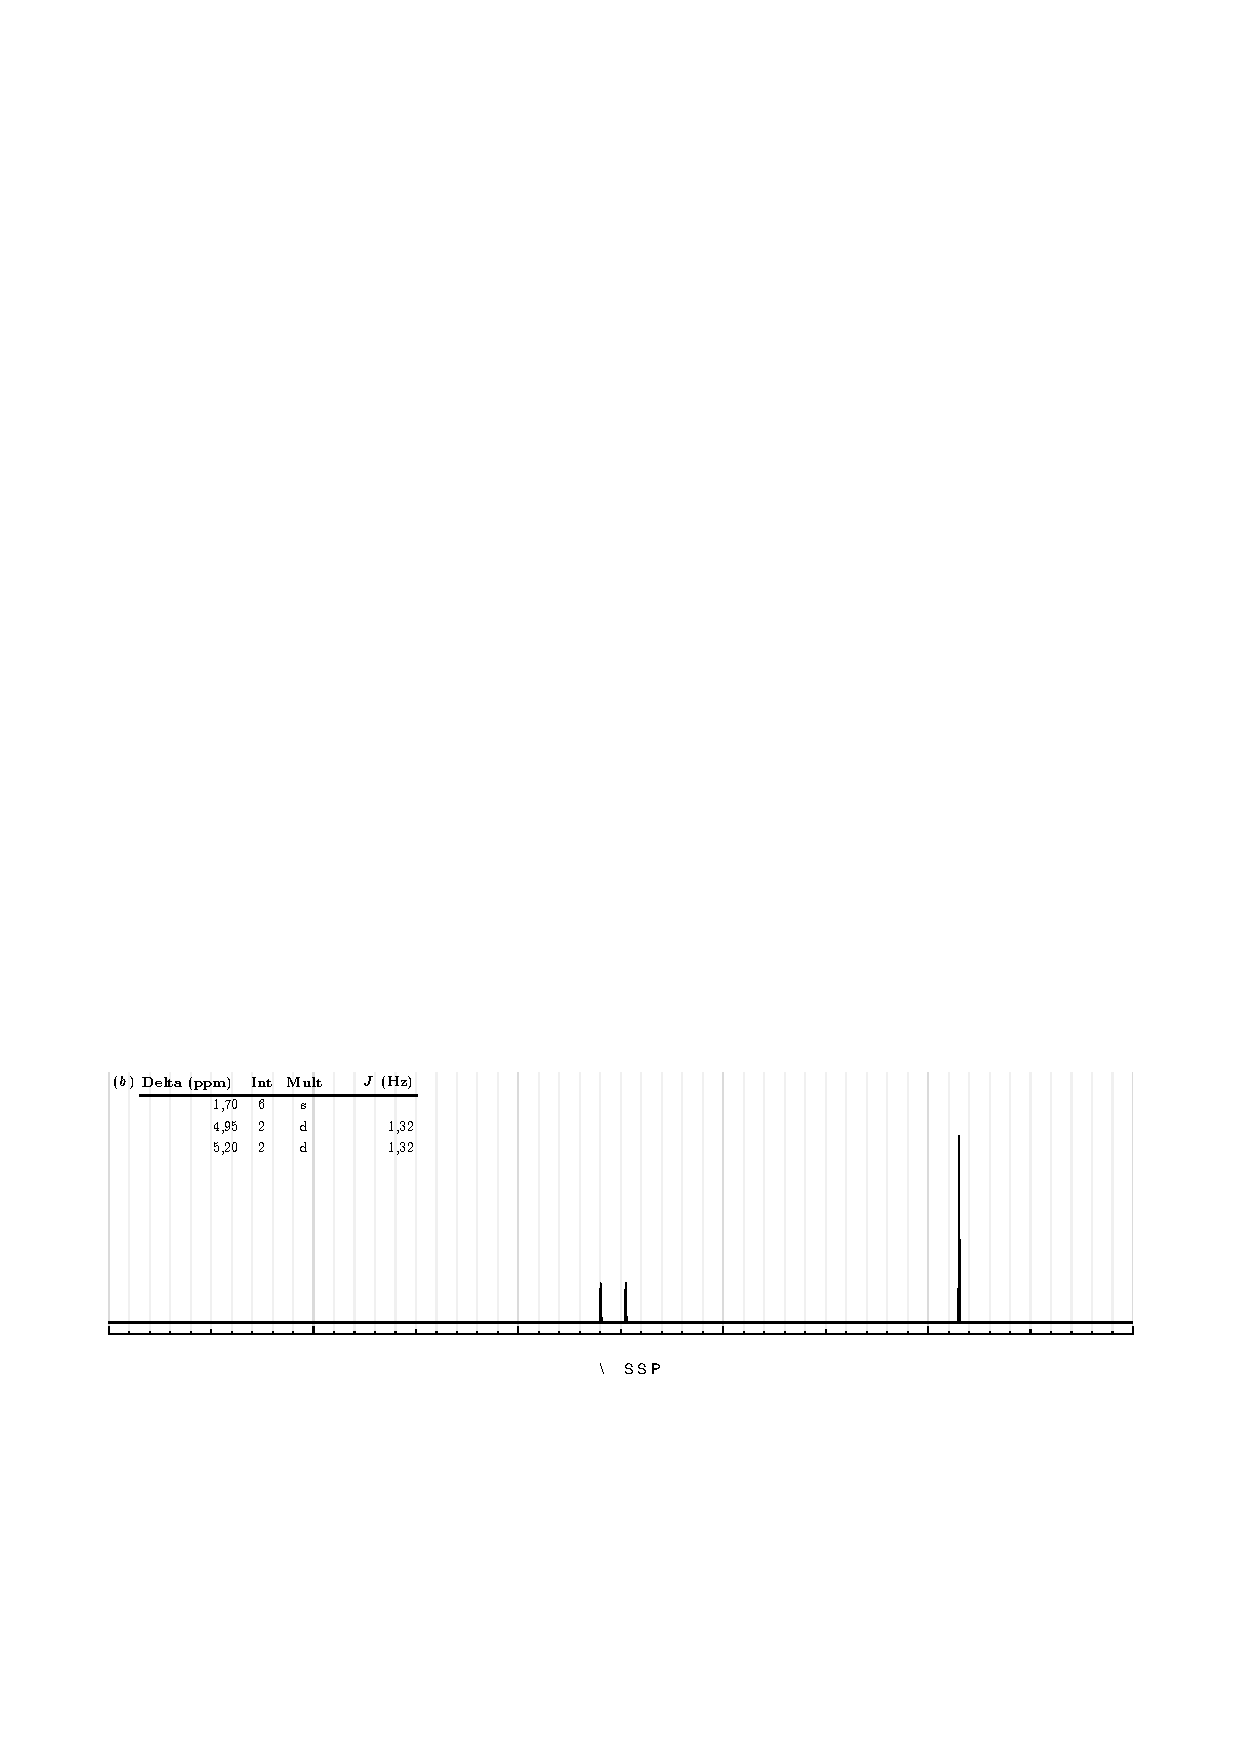
\includegraphics[width=.95\linewidth]{chimiePC/orga/RMN_23.pdf}
    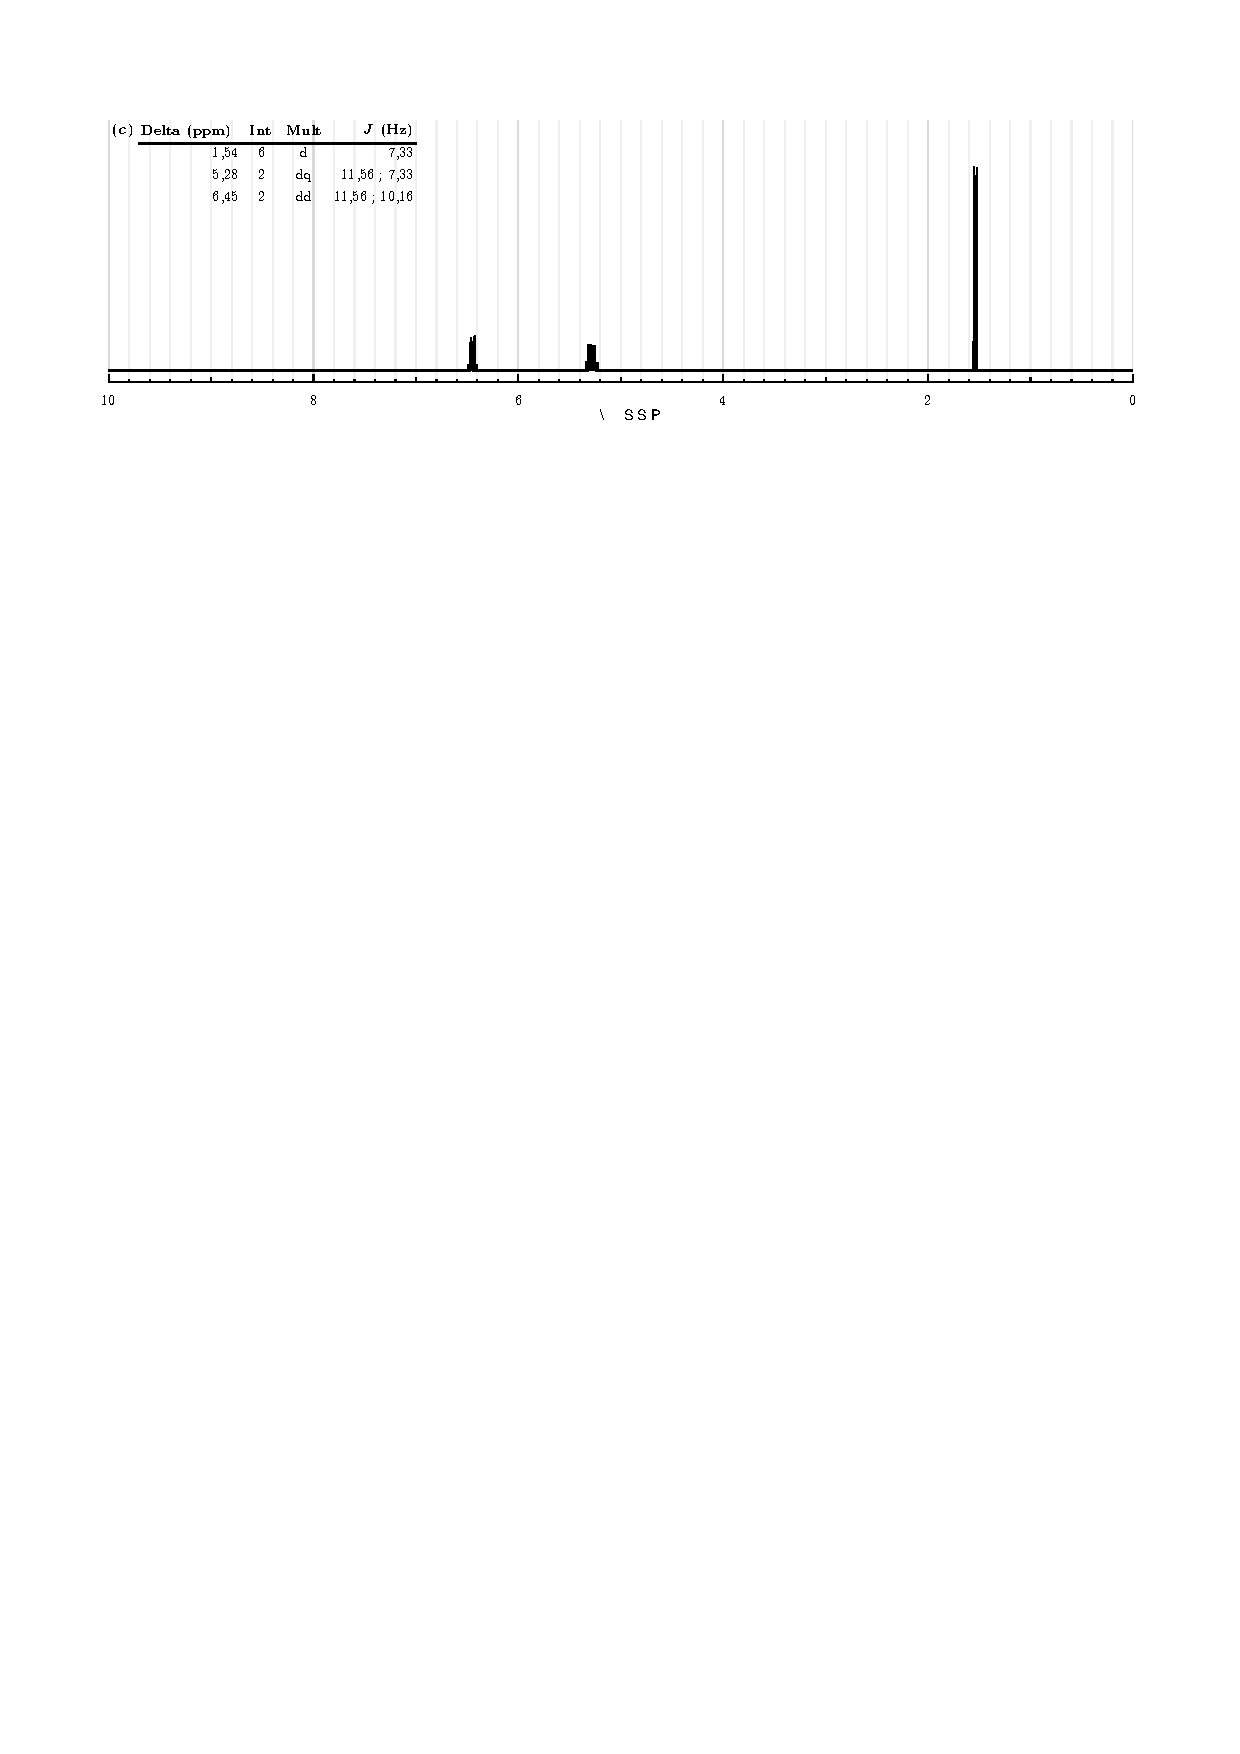
\includegraphics[width=.95\linewidth]{chimiePC/orga/RMN_ZZ.pdf}
    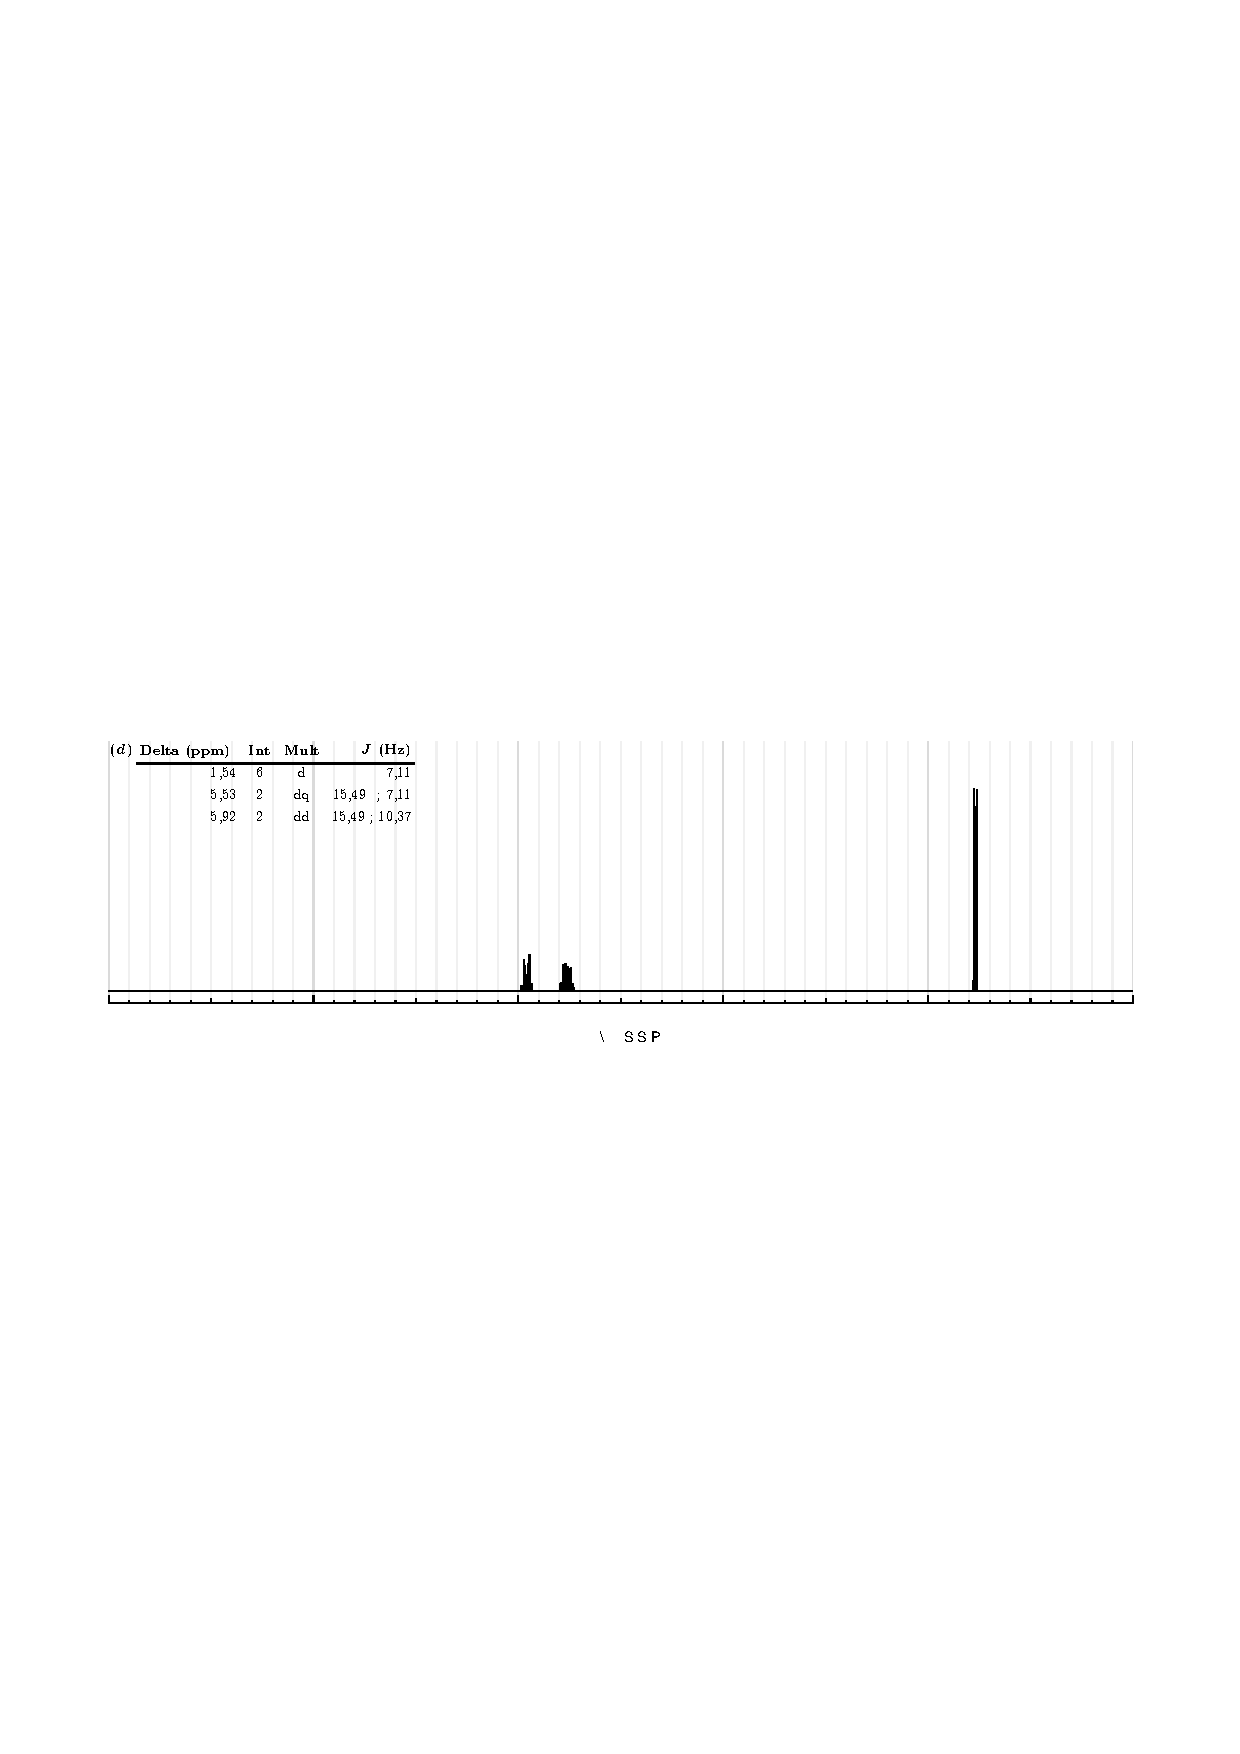
\includegraphics[width=.95\linewidth]{chimiePC/orga/RMN_EE.pdf}
    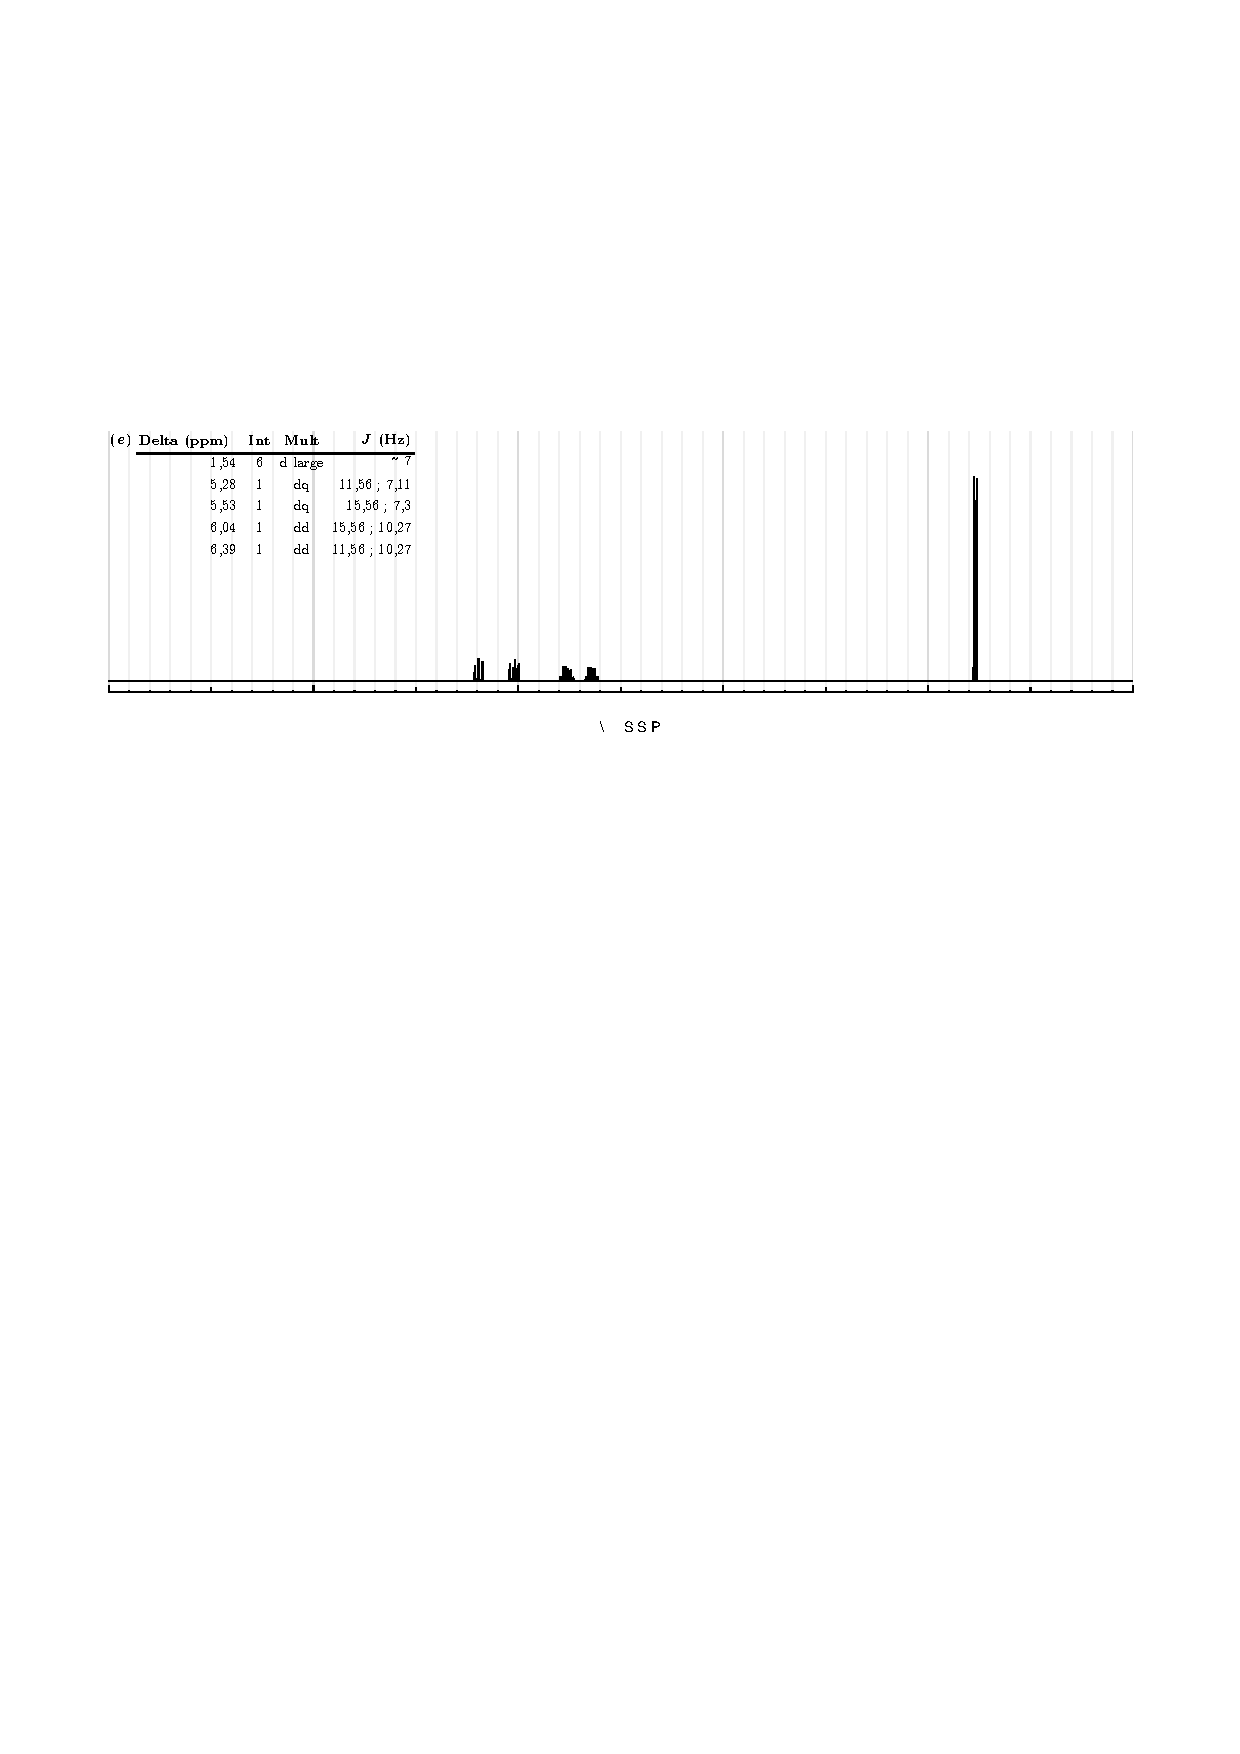
\includegraphics[width=.95\linewidth]{chimiePC/orga/RMN_ZE.pdf}
    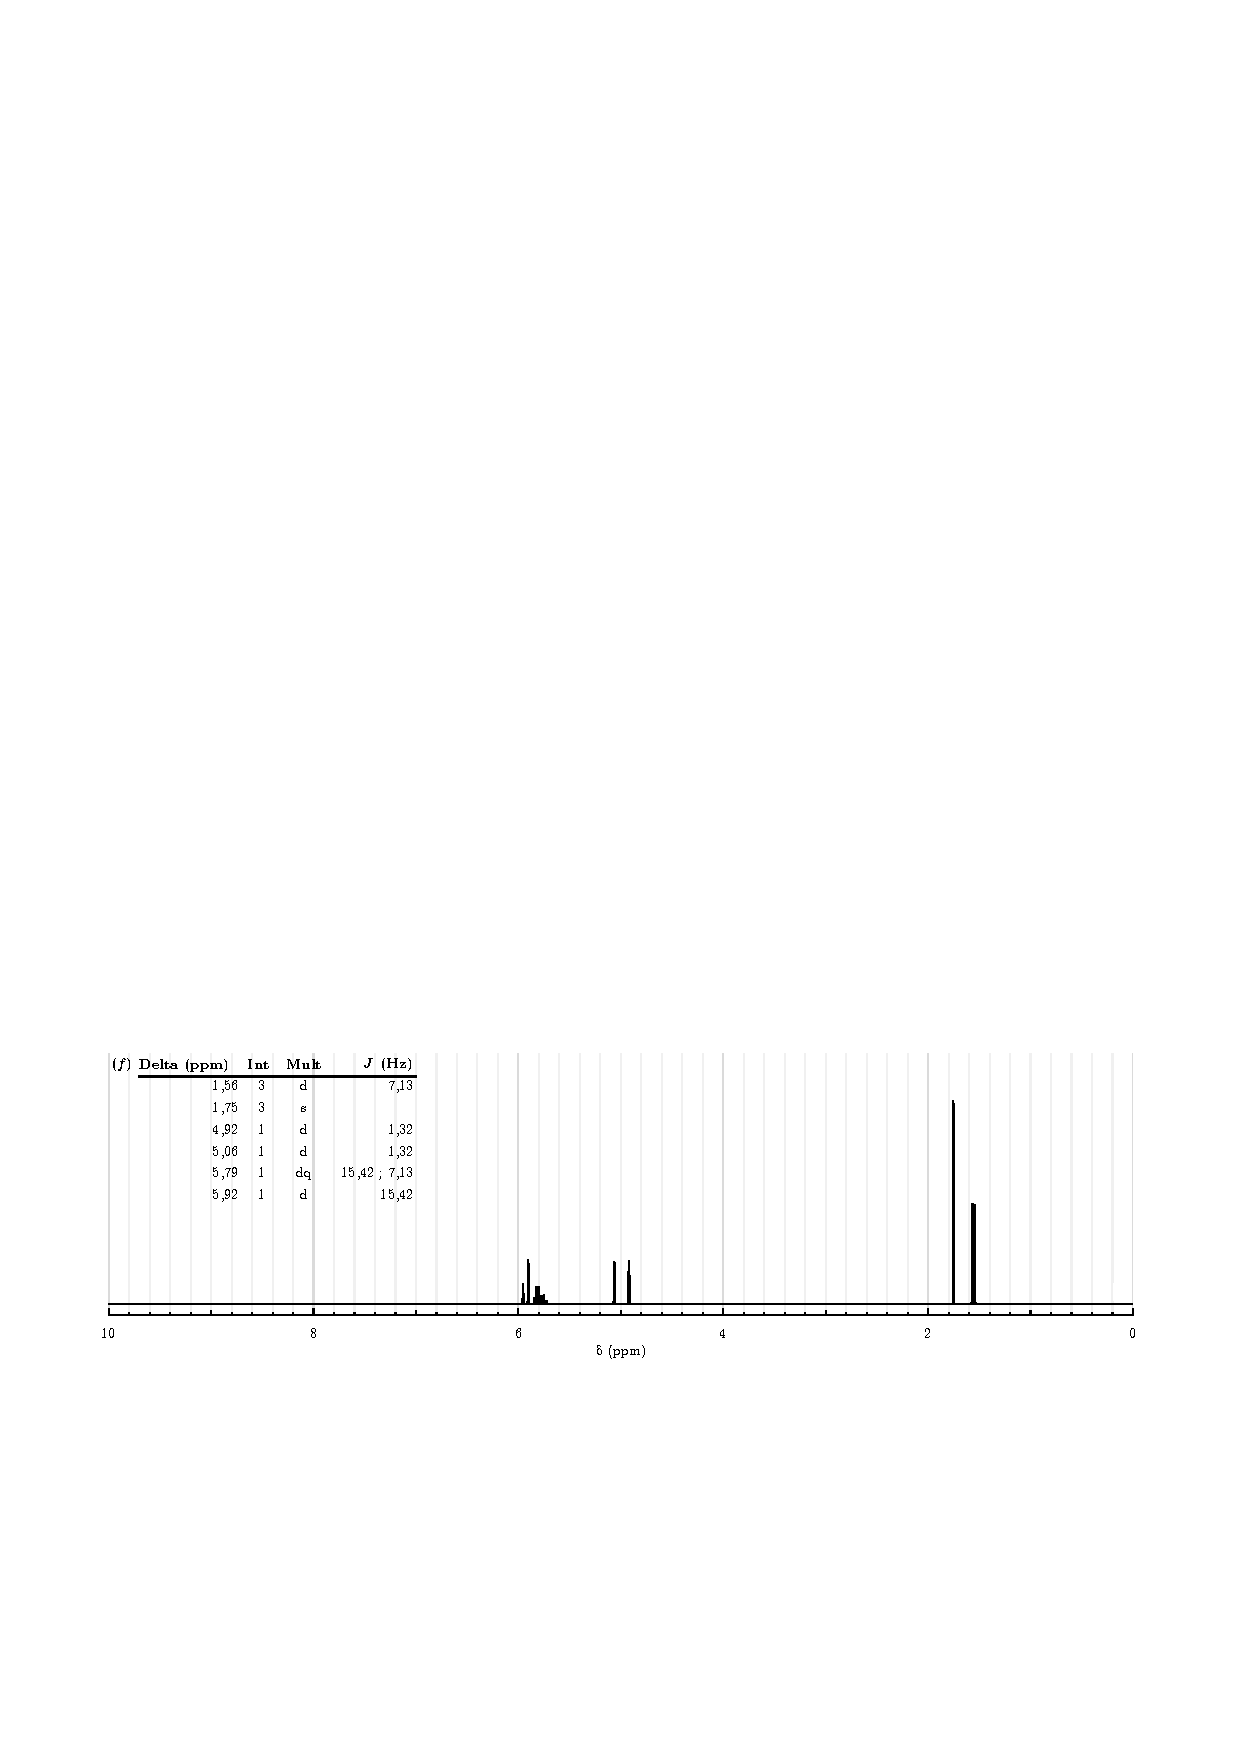
\includegraphics[width=.95\linewidth]{chimiePC/orga/RMN_3E-2.pdf}
    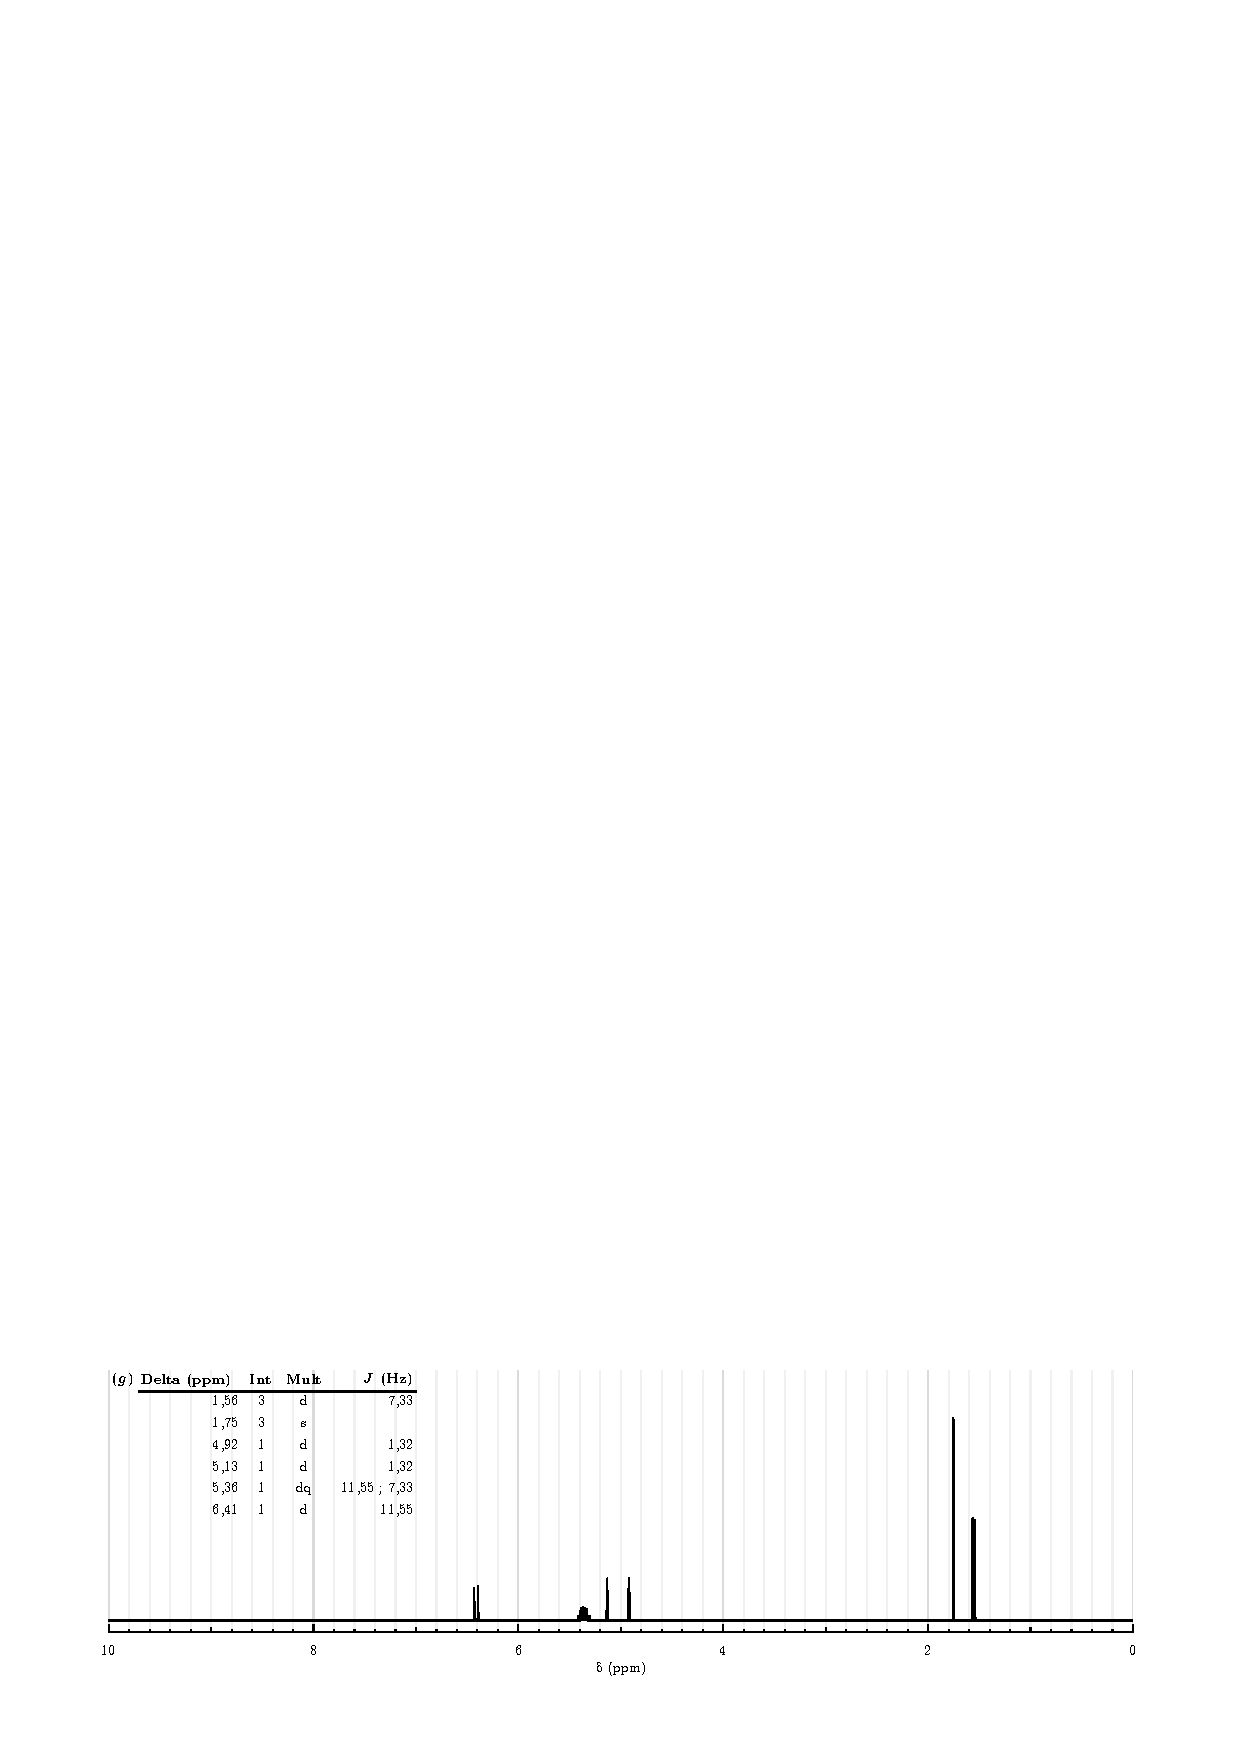
\includegraphics[width=.95\linewidth]{chimiePC/orga/RMN_3Z-2.pdf}
    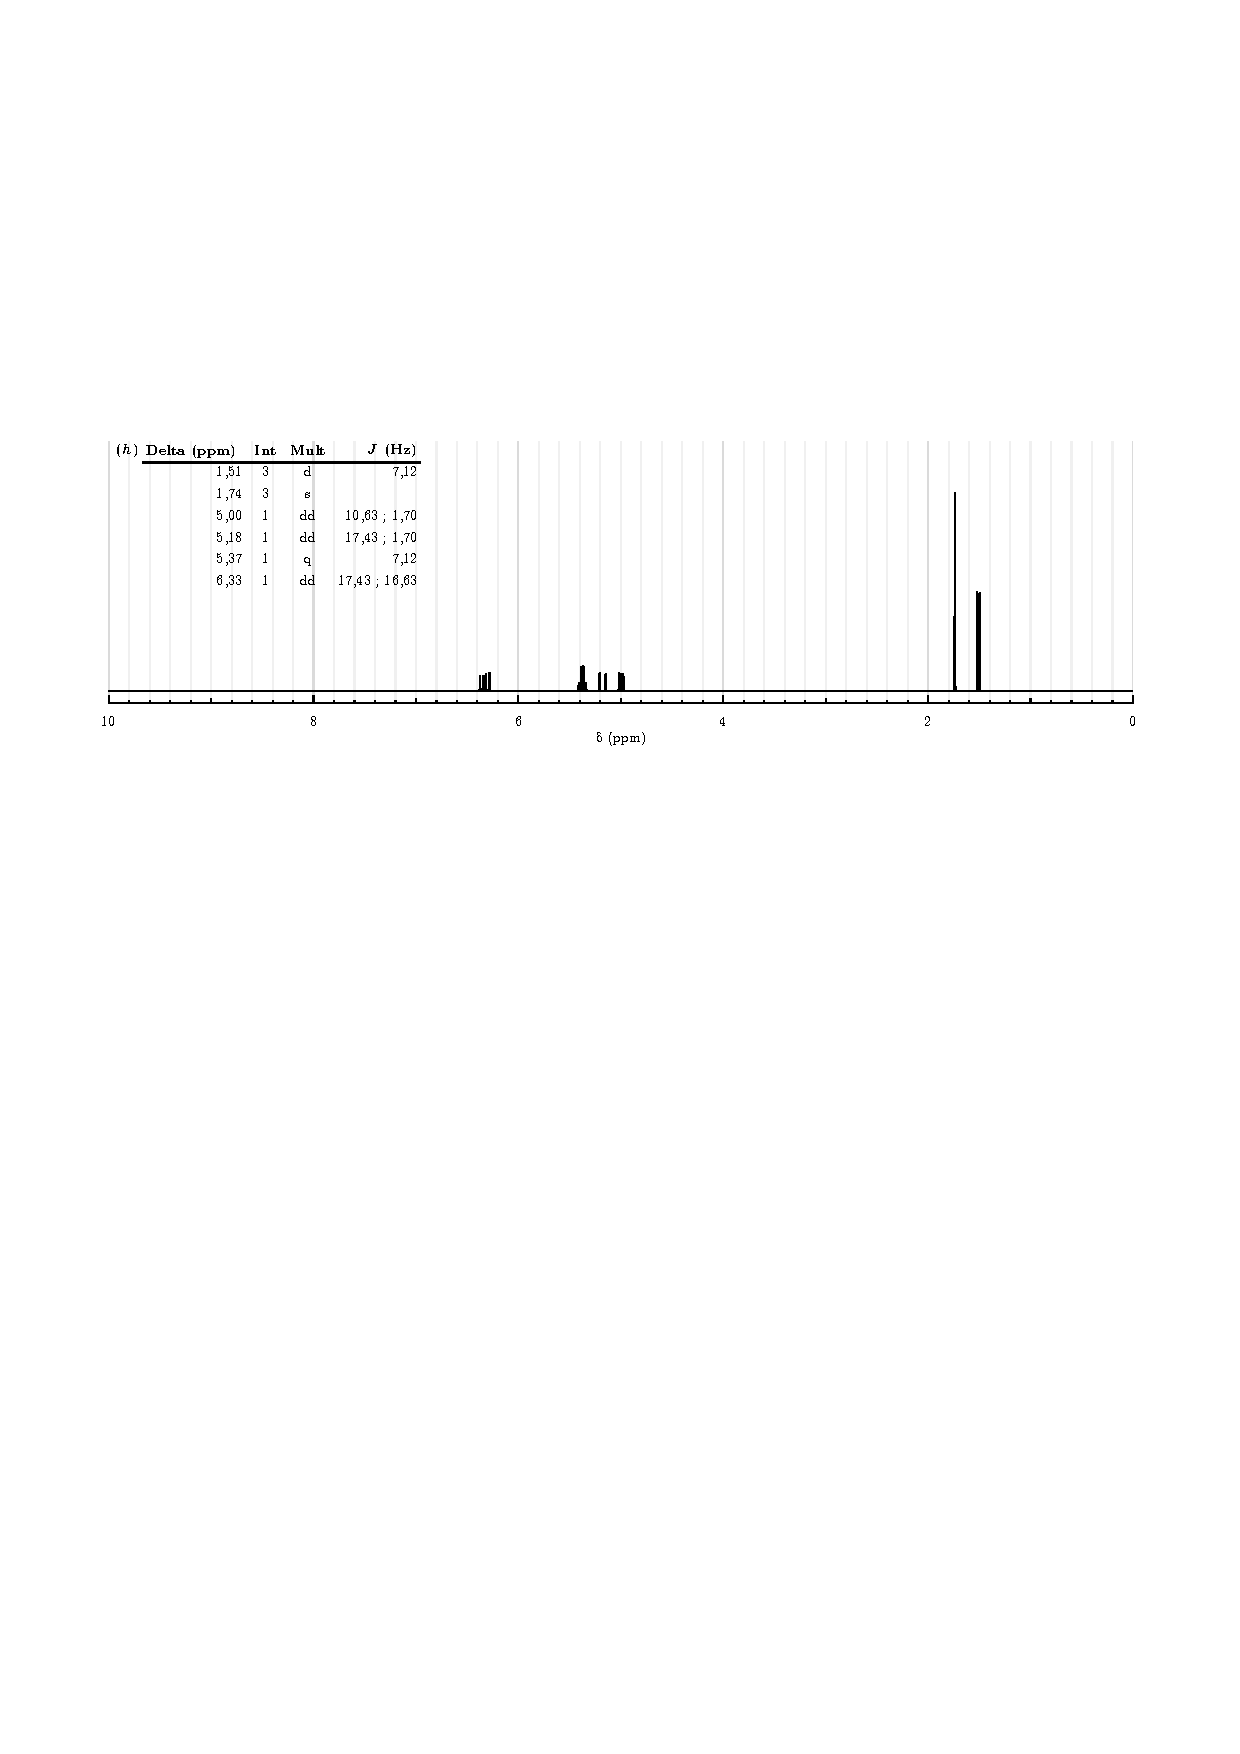
\includegraphics[width=.95\linewidth]{chimiePC/orga/RMN_3E-3.pdf}
    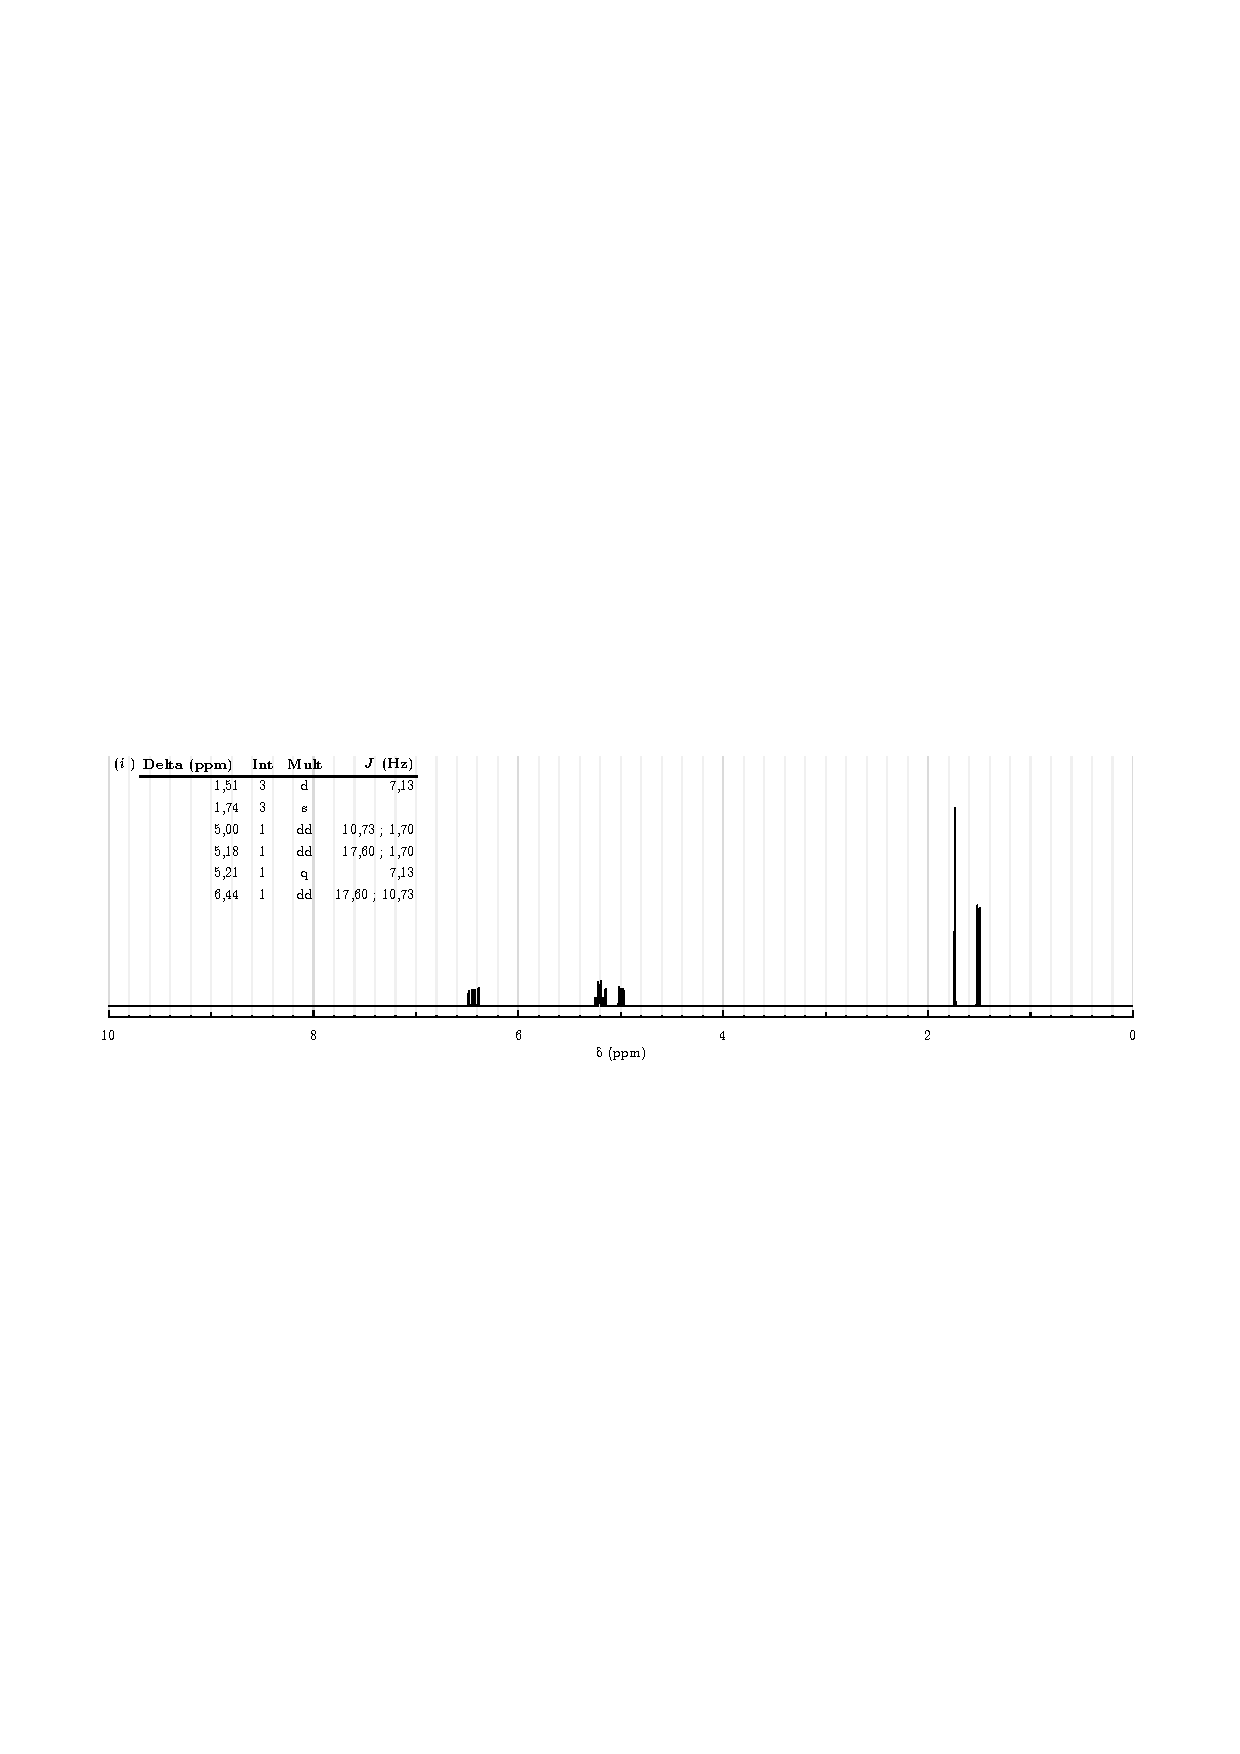
\includegraphics[width=.95\linewidth]{chimiePC/orga/RMN_3Z-3.pdf}
\end{center}

\begin{solution}
\begin{questions}
    \questioncours Multiplicité, topicité...
    
    \question 
    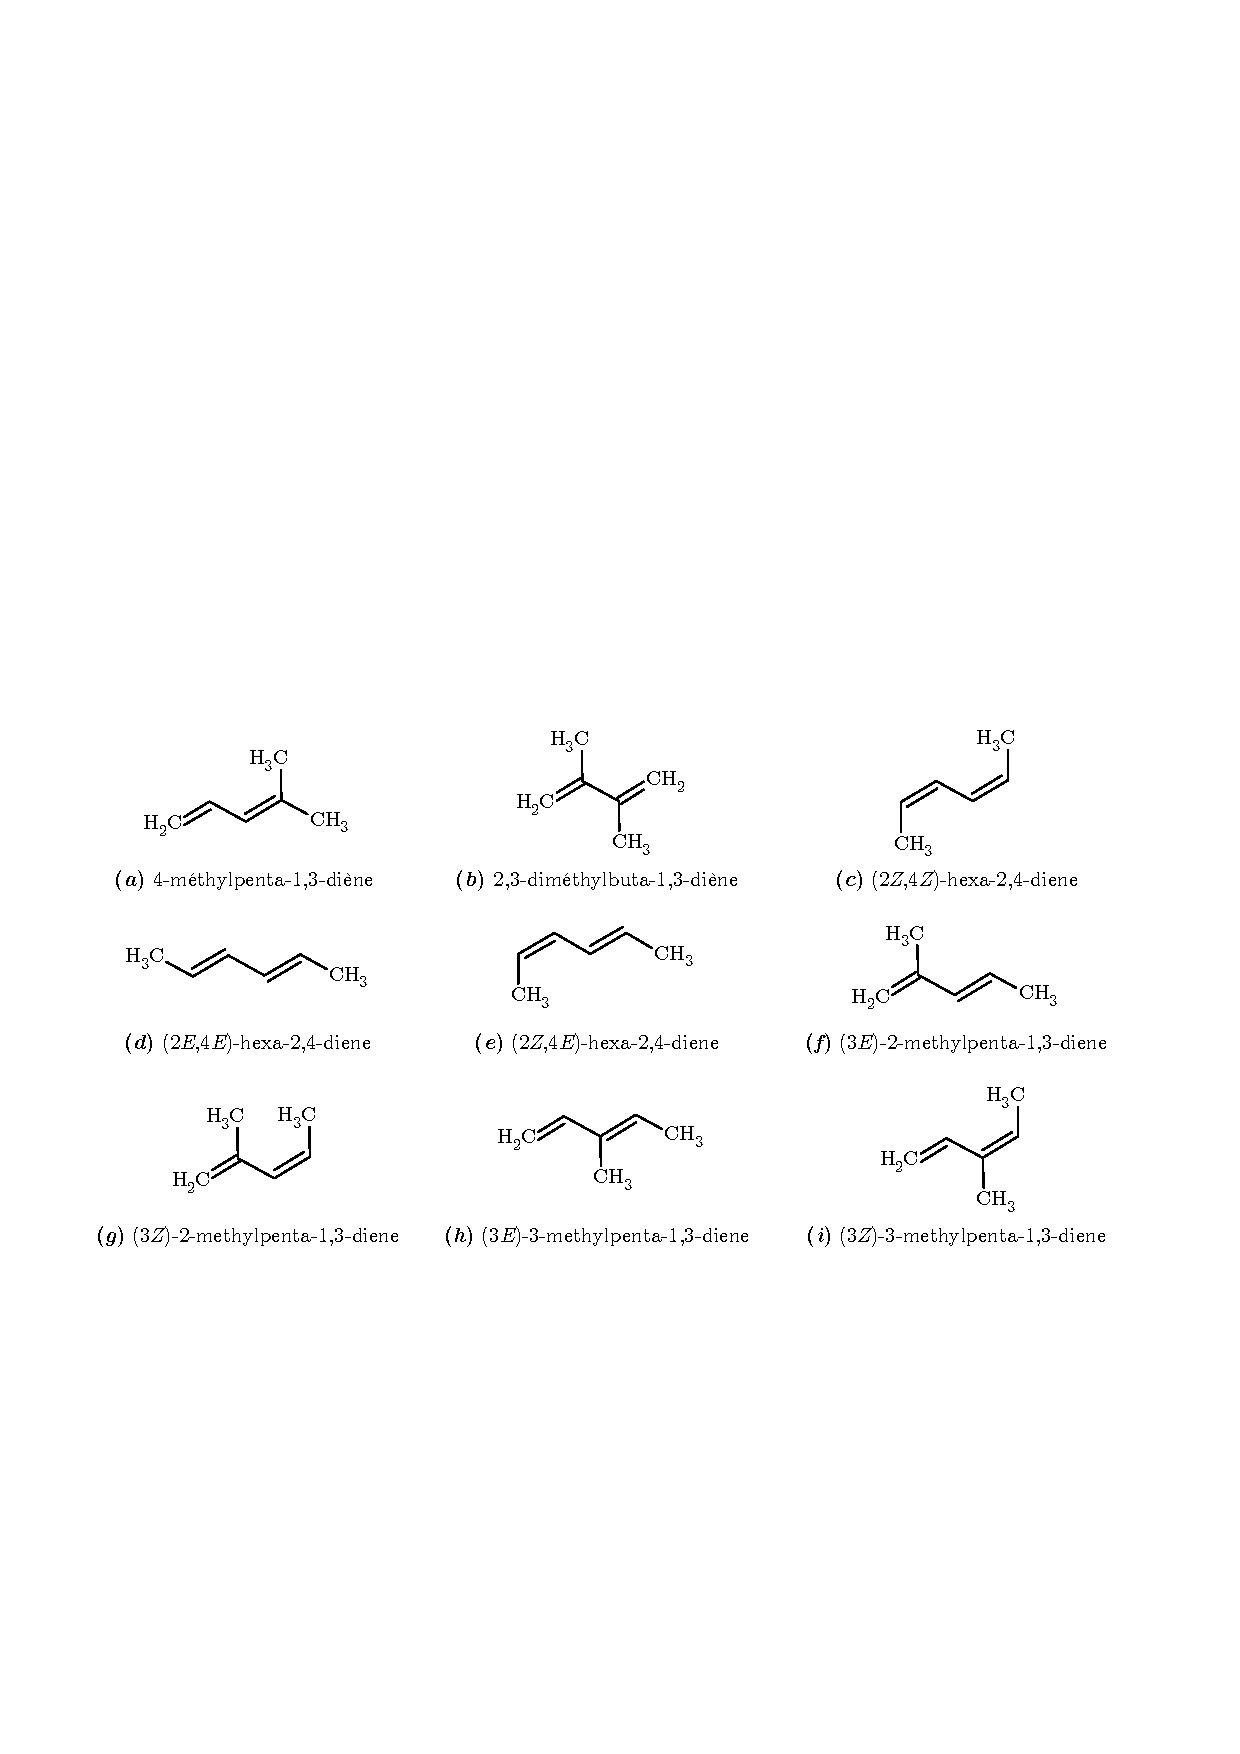
\includegraphics[width=.99\linewidth]{chimiePC/orga/RMN_sols.pdf}
\end{questions}
\end{solution}